\section{Hardware}

After production, the PCB was tested to check it matched the required design.

\subsection{Problems}
\label{ssec:testHWprobs}
Unfortunately, at this point a few issues became apparent.
The first of these was a footprint error.
Due to an error in design the footprint for the OP-AMPs was set to TSOP8, whereas the actual footprint of the component was SOP8.
These footprints are so significantly different there was no way to make the components use the footprint, as such they were unpopulated.
An alternative was sourced, however time and cost constraints prevented them actually being put to use.
\\
\\
The next problem to be discovered was that the fact that the DSP had no on-board flash had not been accounted for.
This was not a major issue as the DSP is capable of running from code in the RAM.
However, actually programming the flash was also an issue.
Both urJTAG and OpenOCD were experimented with, neither with much success.
After a short amount of time it was decided that fighting with the programming capabilities were secondary to getting the algorithm working, and as time was limited it was decided to leave the programming, and come back to it at a later date if time presented itself.
\\
\\
To begin with there was also a short in the power management section.
This was discovered to be a misinterpretation of the pinout of the voltage regulators, resulting in the output voltage being connected directly to the ground plane through the additional pin.
This issue was solved by removing the tracks between the pad for that pin, and the ground plane.

\subsection{Results}
Despite the aforementioned problems in production, many parts of the PCB could still be tested.
\\
\\
The test conditions as shown in table \ref{tab:testconditions} were used for all the tests:

\begin{table}[H]
	\centering
	\begin{tabular}[c]{| l | l | c |}
		\hline
		\multicolumn{2}{|l|}{Factor}		& Value	\\
		\hline
		\multicolumn{2}{|l|}{Voltage}		& 5.00V	\\
		\multicolumn{2}{|l|}{Current Limit}	& 800mA	\\
		\hline
		\multirow{4}{*}{J105}	& $DV_{dd}$	& Unconnected	\\
					& $CV_{dd}$	& Unconnected	\\
					& Codec		& Unconnected	\\
					& Amp		& Unconnected	\\
		\hline
		\multirow{4}{*}{J106}	& Right		& Unconnected	\\
					& Middle Right	& Unconnected	\\
					& Middle Left	& Unconnected	\\
					& Left		& Unconnected	\\
		\hline
		\multirow{4}{*}{J107}	& Right		& Unconnected	\\
					& Middle Right	& Unconnected	\\
					& Middle Left	& Unconnected	\\
					& Left		& Unconnected	\\
		\hline
		\multirow{4}{*}{J108}	& Right		& Unconnected	\\
					& Middle Right	& Unconnected	\\
					& Middle Left	& Unconnected	\\
					& Left		& Unconnected	\\
		\hline
		\multicolumn{2}{|l|}{CONN401}		& Unconnected	\\
		\hline
	\end{tabular}
	\caption{The conditions used in testing}
	\label{tab:testconditions}
\end{table}


\subsubsection{Power}
Firstly the power circuitry was tested.
This was achieved by connecting a bench power supply to the voltage inputs, and measuring the output voltage from the regulators using a digital oscilloscope.
Table \ref{tab:powisotest} shows the results.
The voltage level on the external side of the header was also tested, to check that power wasn't being shorted across.

\begin{table}[H]
	\centering
	\begin{tabular}[c]{| l | c | c |}
		\hline
		Conn		& VR Out (V)	& SC Pin (mV)	\\
		\hline
		$DV_{dd}$	& 3.28		& 190		\\
		$CV_{dd}$	& 1.21		& 37		\\
		Codec		& 3.28		& 34		\\
		Amp		& 3.28		& 32		\\
		\hline
	\end{tabular}
	\caption{The voltages provided by the power circuitry}
	\label{tab:powisotest}
\end{table}

\noindent These results show that the desired voltages were produced.
There was clearly some noise on the external side of the system, however this was low enough to not power up any of the devices.
\\
\\
Another important part of this test was the LED to indicate when the system was powered.
For as long as power was provided to the system this LED stayed lit, as desired.

\subsubsection{DSP}
As discussed in section \ref{ssec:testHWprobs} the DSP was not programmable by the end of the project, this limited the testability of the supporting circuitry.
One test that was possible was simply to power up the DSP, both core and I/O, and check that there were no short circuits.
In order to test this the conditions shown in table \ref{tab:dsptestconditions} were used.

\begin{table}[H]
	\centering
	\begin{tabular}[c]{| l | l | c |}
		\hline
		\multicolumn{2}{|l|}{Factor}		& Value	\\
		\hline
		\multirow{4}{*}{J105}	& $DV_{dd}$	& Connected	\\
					& $CV_{dd}$	& Connected	\\
					& Codec		& -		\\
					& Amp		& -		\\
		\hline
	\end{tabular}
	\caption{Conditions for testing the DSP}
	\label{tab:dsptestconditions}
\end{table}

\noindent The conclusion of this test was simply that there were no short circuits, as the power supply did not current limit.
TODO: Get JTAG chip details, proof of JTAG functionality.

\subsubsection{Codec}
Unfortunately, without being able to program the DSP it is not possible to configure the codec to interact.
However, there is a second part to that circuit that can be tested, the clock generator.
In order to test this, the codec circuitry was powered up by setting the headers as shown in table \ref{tab:codectestconditions}.

\begin{table}[H]
	\centering
	\begin{tabular}[c]{| l | l | c |}
		\hline
		\multicolumn{2}{|l|}{Factor}		& Value	\\
		\hline
		\multirow{4}{*}{J105}	& $DV_{dd}$	& -		\\
					& $CV_{dd}$	& -		\\
					& Codec		& Connected	\\
					& Amp		& -		\\
		\hline
	\end{tabular}
	\caption{Conditions for testing the Codec}
	\label{tab:codectestconditions}
\end{table}

\noindent When tested the output of the clock generator produced the waveform in figure \ref{fig:codec12Mclk}.
This shows that the clock generator was producing a $12MHz$ square wave signal as desired.
This signal was between $0-3.3V$ as required by the codec inputs, however reached $5V_{pk-pk}$ which would not have been acceptable by the codec.
In order to resolve this issue a small capacitor could be placed in parallel with the output of the clock generator.
This would serve the purpose of removing the ripples on the signal and keep it within the bounds required by the codec.

\begin{figure}[H]
	\centering
	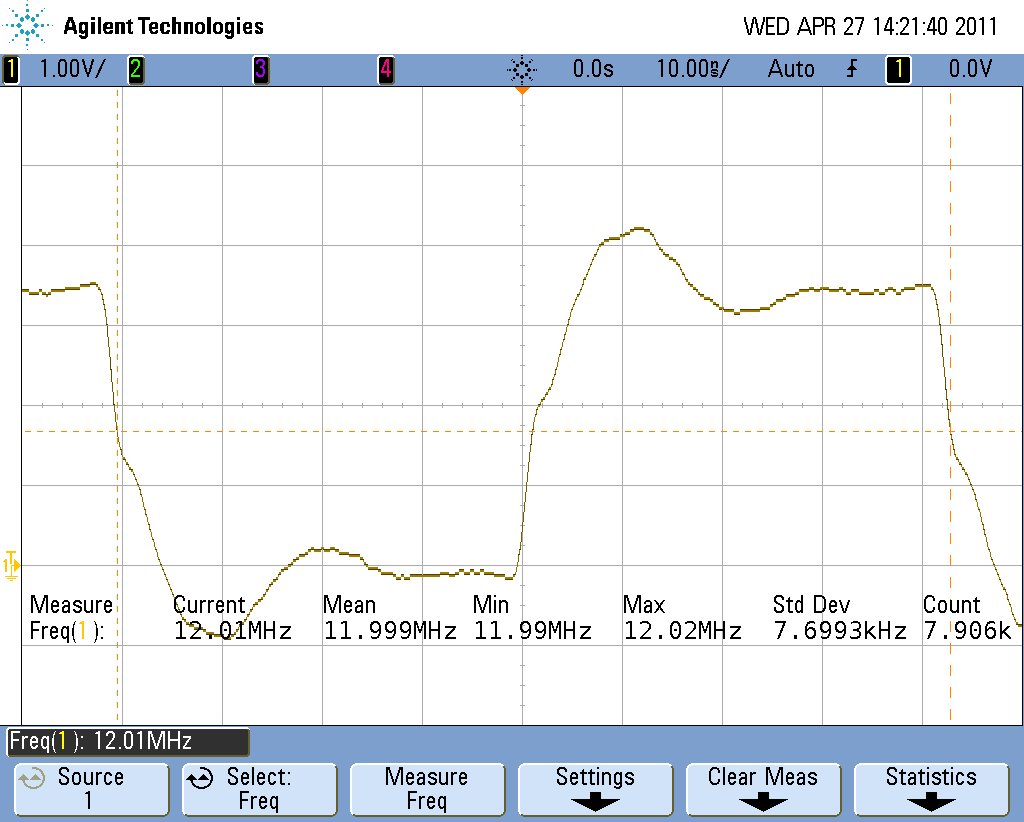
\includegraphics[width=\textwidth]{./img/codec_12M_clk.png}
	\caption{Output waveform of the clock generator}
	\label{fig:codec12Mclk}
\end{figure}

\subsubsection{Analogue}

